In this section we describe the design of Cerebro, our system for establishing response time SLAs for
cloud APIs. We explain its major components, their interactions and how the 
system works as a whole. Recall that the overarching theme of our approach is to combine program
static analysis with cloud platform monitoring to formulate an accurate performance model for the 
web APIs developed for a given cloud platform. Therefore, at very least Cerebro requires the following 
two components:

\begin{itemize}
\item A program static analysis component that can extract the sequence of cloud SDK operations invoked by a web API
code.
\item A monitoring agent that runs in the target cloud platform to monitor the performance of its individual cloud SDK
operations.
\end{itemize}
 
 \subsection{Program Static Analysis Component}
 The static analysis component analyzes the source code (or some intermediate representation of it), to identify
 the cloud SDK operations invoked by a given web API code. Since a web API code can only make a finite
 number of cloud SDK invocations, and since PaaS clouds only support a finite number of cloud
 SDK operations, it is possible to design an algorithm that
 extracts all cloud SDK invocations from any given web API code. 

The basic idea behind Cerebro's static analysis is to construct and walk the
 control flow graph (CFG)~\cite{Allen:1970:CFA:800028.808479} of the given code. Whenever the 
 algorithm encounters a node that represents a function call,
 it checks whether the function call corresponds to a cloud SDK operation. If so the algorithm
adds it to the output of the analysis. At the end of the analysis, the algorithm outputs a list whose members are
sequences of cloud SDK operations. Each sequence of operations corresponds to a different
path of execution through the code.

Listing 1 shows the outline of the basic program analysis algorithm used by Cerebro. 
Constructing the CFG from a given program is a common requirement
in program analysis, and there are several well-understood mechanisms to implement it~\cite{Aho:1986:CPT:6448,Morgan:1998:BOC:288765,Muchnick:1998:ACD:286076}. 
CFG traversal is performed in the depth-first 
fashion to ensure that the algorithm walks each path of execution to the end of the program, before picking up on
a new path. The algorithm marks the nodes in the CFG as it visits them to ensure that the graph traversal does not 
get stuck in loops. 

If the algorithm detects any function call nodes that correspond to functions in the user's code, the algorithm
starts analyzing the code of the target functions recursively. This effectively turns our analysis into an inter procedural
CFG analysis. Results obtained from analyzing user-implemented functions can be cached to avoid
having to analyze the same function more than once. Note that the algorithm simply appends the results of
analyzing user-implemented functions to the current sequence of cloud SDK invocations. This ensures that the final output of the
analysis contains cloud SDK invocation sequences spanning across all the relevant functions in the code. 
In other words, the sequences in the final output may cross function boundaries.
Since any web API implementation must have a finite amount of code, as long as
we mark the visited nodes in the CFG (to handle loops), and keep track of the functions that we have 
already analyzed or have begun to analyze (to handle recursion), this analysis is guaranteed to terminate with results.

In Cerebro we do not recursively analyze any of the cloud
SDK operations or any third party library calls. 
Statically analyzing the internals of cloud SDK invocations is
unnecessary since we intend to build a performance model for web APIs where
the smallest unit of operation is a cloud SDK call. As for third 
party libraries, we assume they do not contain any cloud SDK invocations -- a reasonable assumption 
regarding most third party libraries that are generic and intended to run on a variety of target runtimes. 
 
%Cerebro's static analysis is mostly comprised of well-understood, general purpose program analysis techniques.
Perhaps the only application-specific element in our algorithm is the method used to check function call nodes for cloud SDK invocations.
 In the worst case this check can be implemented as a table lookup. That is, we maintain a table of all possible cloud
 SDK operations, and check whether each function call
 corresponds to an entry in the table. In real world implementations there are other more efficient methods that
 can be employed to solve this problem. For instance some PaaS clouds use a special naming convention to label
 their cloud SDK operations. 
 In such a scenario we can simply check whether the function calls in CFG nodes match the
 desired pattern. 
 
The algorithm in listing 1 is only meant as an outline for a minimalistic program analysis.
We incorporate more sophisticated analyses into this algorithm to extract more
useful information regarding the cloud SDK invocations. For example, we perform a loop extraction on the
CFG to identify the loops in the code, and tag the cloud SDK invocations in the output to indicate which of them
are executed inside loops. In such an implementation, the output of the static analysis will not be a simple
list of cloud SDK invocation sequences. Rather, it will be a list of \textit{annotated} cloud SDK invocation sequences.

When there are cloud SDK invocations present inside loops, it would be useful to know how many times those loops
are going to execute. Any performance model based on cloud SDK calls made by a web API code,
needs to account for the repeated execution of cloud SDK calls inside loops. If the 
loops in question are data-independent (i.e. the iteration count does not depend on the size of the data processed 
by the code), we use a static loop bound estimator to determine how many times the loops are going to iterate~\cite{bygde2010static,Gulwani:2009:CRP:1542476.1542518,Lokuciejewski:2009:FPS:1545006.1545064,Hunt:2006:PCL:1167999.1168026}.
This is done for each loop extracted during our CFG analysis, and the estimated loop bounds can be added to the
analysis output as annotations.

However, as indicated by our survey results, loops are fairly uncommon in web API codes developed for PaaS clouds. When
they are present, they usually iterate over some dataset (i.e. data-dependent). Such loops cannot
be accurately predicted using static analysis methods. But survey results also show us that
most of the time cloud web API codes iterate over datasets loaded from the underlying datastore of the PaaS.
We use this as a heuristic to bound the iteration count of data-dependent loops. Typically, application developers
have an approximate idea of how large their database will be once their code is in production. When we encounter a data-dependent
loop in the CFG that we cannot accurately predict using a static loop bound estimator, we simply
prompt the developer to enter a reasonable maximum size for the underlying database (i.e. the maximum number of
records/entities that may be returned from the datastore). We
use these developer-specified values as upper bounds for the loop iteration count. 
This information is also added to the final outcome of the static analysis as annotations.

\subsection{Watchtower: Cloud Platform Monitoring Agent}
Watchtower is the Cerebro component that tracks the performance of individual
cloud SDK operations over time. This component can be an integral part of the PaaS cloud that
monitors cloud SDK operations from within, or it can be another application deployed on the PaaS
that periodically benchmarks the cloud SDK operations from the outside. Regardless of how it is
implemented, it must cater for two requirements:

\begin{itemize}
\item Watchtower should always be active, and collect data as long as the cloud platform is available for serving web API requests.
\item Watchtower should periodically measure the time taken by individual cloud SDK operations, and arrange the gathered data into time series (one time series per cloud SDK operation).
\end{itemize}

In addition to the above requirements, Watchtower should also expose some web APIs of its own 
so that other components in Cerebro can query the Watchtower to retrieve the collected time series data. Also,
it should keep the collected time series data in a persistence storage for durability. The most logical
place to store this data would be the underlying datastore of the PaaS itself, since it is already designed
for high scalability. To avoid unbounded accumulation of time series data, Watchtower can discard the old
measurements once a certain amount of time has elapsed. 
%For example, it can periodically clean up
%all data points that are more than a month old. It is fair to assume that the current performance of web APIs
%is not influenced by how the cloud SDK operations behaved a month ago.

The frequency at which
Watchtower collects data determines how often Cerebro can generate SLA predictions for web APIs. Practically
speaking, it is sensible to benchmark the cloud SDK operations once every few minutes (i.e. 1-10 minutes). It does not make
sense to collect data any more frequently than that, since we naturally expect each predicted SLA to 
hold correct for a time period longer than a few minutes.

In order to make SLA predictions regarding codes that include data-dependent loops, Watchtower
benchmarks some common iterative cloud SDK operations. 
Watchtower executes a series of iterative datastore reads,
while varying the result set size, to measure the time required to loop through different sized result sets. These
measurements are also stored as time series data, where each result set size gets its own time series. 
It is not necessary to benchmark all possible result set sizes. Rather, Watchtower should only benchmark a
handful of result set sizes  (e.g. 1, 1000 and 1000000 records) that are representative of common 
production workloads.

\subsection{Making SLA Predictions}
%So far we have explained our approach for statically analyzing the web API codes to extract the sequence
%of cloud SDK operations, and periodically benchmarking the performance of individual cloud SDK
%operations. Next step is to combine these two pieces of information and predict the execution time of the
%web API code. For this purpose we employ an existing machine learning technique called
%QBETS (Queue Bounds Estimation from Time Series)~\cite{Nurmi:2007:QQB:1791551.1791556}. 

To make SLA predictions, Cerebro uses QBETS (Queue Bounds Estimation from Time Series)~\cite{Nurmi:2007:QQB:1791551.1791556},
a non-parametric time series analysis method.
%QBETS looks at past time series data, and predicts
%an upper bound on a specific percentile at a fixed level of confidence. 
It was originally designed for
predicting the scheduling delays on batch queue systems used in high performance computing (HPC) environments. 
We adapt this technique for predicting the execution time of API codes.

A QBETS analysis requires three inputs:
\begin{enumerate}
\item A time series of data generated by a continuous experiment
\item The percentile for which an upper bound should be predicted ($p \in [1..99]$)
\item The upper confidence level of the prediction ($c \in (0,1)$)
\end{enumerate}

QBETS uses this information to predict an upper bound for the $p$-th percentile of the time series.
The predicted value has a probability of $0.01p$ of being greater than or equal to the next data point that
will be added to the time series by the continuous experiment. 
The upper confidence level $c$ serves as a conservative
bound on the predictions. That is, predictions made with an upper confidence level of $c$ will overestimate
the true percentile with a probability of $1-c$. This confidence guarantee is necessary because 
QBETS does not determine the 
percentiles of the time series precisely, but only estimates them. 

To further clarify what QBETS does, assume a continuous experiment that periodically measures the
response time of a web API. This results in a time series of response time data. Suppose at time $t$,
we run QBETS on the time series data collected so far with $p=95$ and $c=0.01$. The prediction returned
by QBETS has a 95\% chance of being greater than or equal to the next response time value measured
by our experiment after time $t$. Since $c=0.01$, the predicted value has a 99\% chance of
overestimating the true 95th percentile of the time series.

We find QBETS to be an ideal fit for our work due to several reasons. 
\begin{itemize}
\item QBETS works with time series data. Since
cloud SDK benchmarking data can be easily represented as time series,
they are highly amenable for QBETS analysis. 
\item QBETS makes predictions regarding the
future outcomes of an experiment by looking at the past outcomes -- an idea that resonates well with our
goal of predicting future API response times from past cloud SDK benchmarking data. 
\item Response time
SLAs of web APIs should be specified with exact correctness probabilities and confidence levels for
them to be useful. Predictions made by QBETS meet these requirements well. 
\item QBETS is 
simple, efficient and has been applied successfully to analyze a wide range of time series data in the past.
%More specifically, it has been tested with both autocorrelating and non-autocorrelating time series data.
\end{itemize}

We now describe our exact algorithm for combining static analysis data with cloud platform monitoring 
data through QBETS. Recall that our static analysis produces a list of cloud SDK invocation sequences.
We start by pruning this list to eliminate duplicates. Duplicates can occur if a web API code has
multiple paths of execution, where more than one path consists of the same exact sequence of cloud 
SDK invocations. Then for each sequence of cloud SDK invocations present in the pruned list, we
perform the following operations:

\begin{enumerate}
\item Retrieve benchmarking data from Watchtower for all operations in the sequence. Watchtower provides
this information as ordered time series data (one time series per cloud SDK operation).
\item Align the retrieved time series so that data points collected at the same time line up against each other.
Add the time series data to form a single aggregate time series for the sequence of cloud SDK operations.
\item Pass the aggregate time series to QBETS along with the desired $p$ and $c$ values to predict an
upper bound for some percentile. 
\end{enumerate}

We shall present a concrete example to further clarify this process. Suppose our static analysis results in the
cloud SDK invocation sequence $<op_{1},op_{2},op_{3}>$. Lets assume Watchtower has the following
time series data collected for the three operations in the sequence.

\begin{itemize}
\item $op_{1}$: $[t_{0}: 5, t_{1}: 4, t_{2}: 6, ...., t_{n}: 5]$
\item $op_{1}$: $[t_{0}: 22, t_{1}: 20, t_{2}: 21, ...., t_{n}: 21]$
\item $op_{1}$: $[t_{0}: 7, t_{1}: 7, t_{2}: 8, ...., t_{n}: 7]$
\end{itemize}

Here $t_{m}$ are timestamp values Watchtower has assigned to each data point. We align the three
time series, so that values with the same timestamp are grouped together, and aggregate the results
to obtain the following time series.

$[t_{0}: 34, t_{1}: 31, t_{2}: 35, ...., t_{n}: 33]$

Then we pass the aggregate time series to QBETS for analysis, and
treat the QBETS prediction as an SLA for the web API code.
If the QBETS predicted value is $Q$ milliseconds, we can form the SLA as ``the web API responds 
under $Q$ milliseconds, $p$ percent of the time''. When the code has multiple paths of execution (and
hence multiple sequences of cloud SDK operations), we can predict more than one SLA for the API. In
such cases we can treat the SLA with highest predicted value as the final SLA (i.e. worst case SLA).

When the static analysis produces cloud SDK invocation sequences with information about loops, we 
need to do some extra work. If some operation has been tagged as being inside a loop, where the loop
bounds have been estimated, the time series data corresponding to that operation should be multiplied 
by the loop bound estimate, before aggregating. In cases where the operation is inside a data-dependent
loop, we can use the developer specified loop bound (e.g. maximum records
in database), to fetch the most appropriate benchmark data from Watchtower.
For example, if a sequence contains an iterative datastore read which has been annotated with a maximum
record count of 1000, we can request Watchtower to provide time series data for the iterative datastore
read operation with a result set size of 1000. When an exact match cannot be found, Watchtower can
provide the results for the closest result set size that is larger than the requested limit.

In order to make a trustworthy prediction, QBETS needs to see a sufficiently large number of data points
in the input time series. In fact it can be proven that QBETS needs to see at least $log(c)/log(0.01p)$ data points
before it can start making highly reliable predictions. This means, if we are interested in predicting the 95th percentile
of the API execution time, with an upper confidence of 0.01, we should feed QBETS with a time series that
contains at least 90 data points. Watchtower should take this into consideration, when garbage collecting old
time series data. That is, it should always keep enough data points so that QBETS have enough data to analyze.

\subsection{Overall Architecture and Workflow}

\begin{figure}
\centering
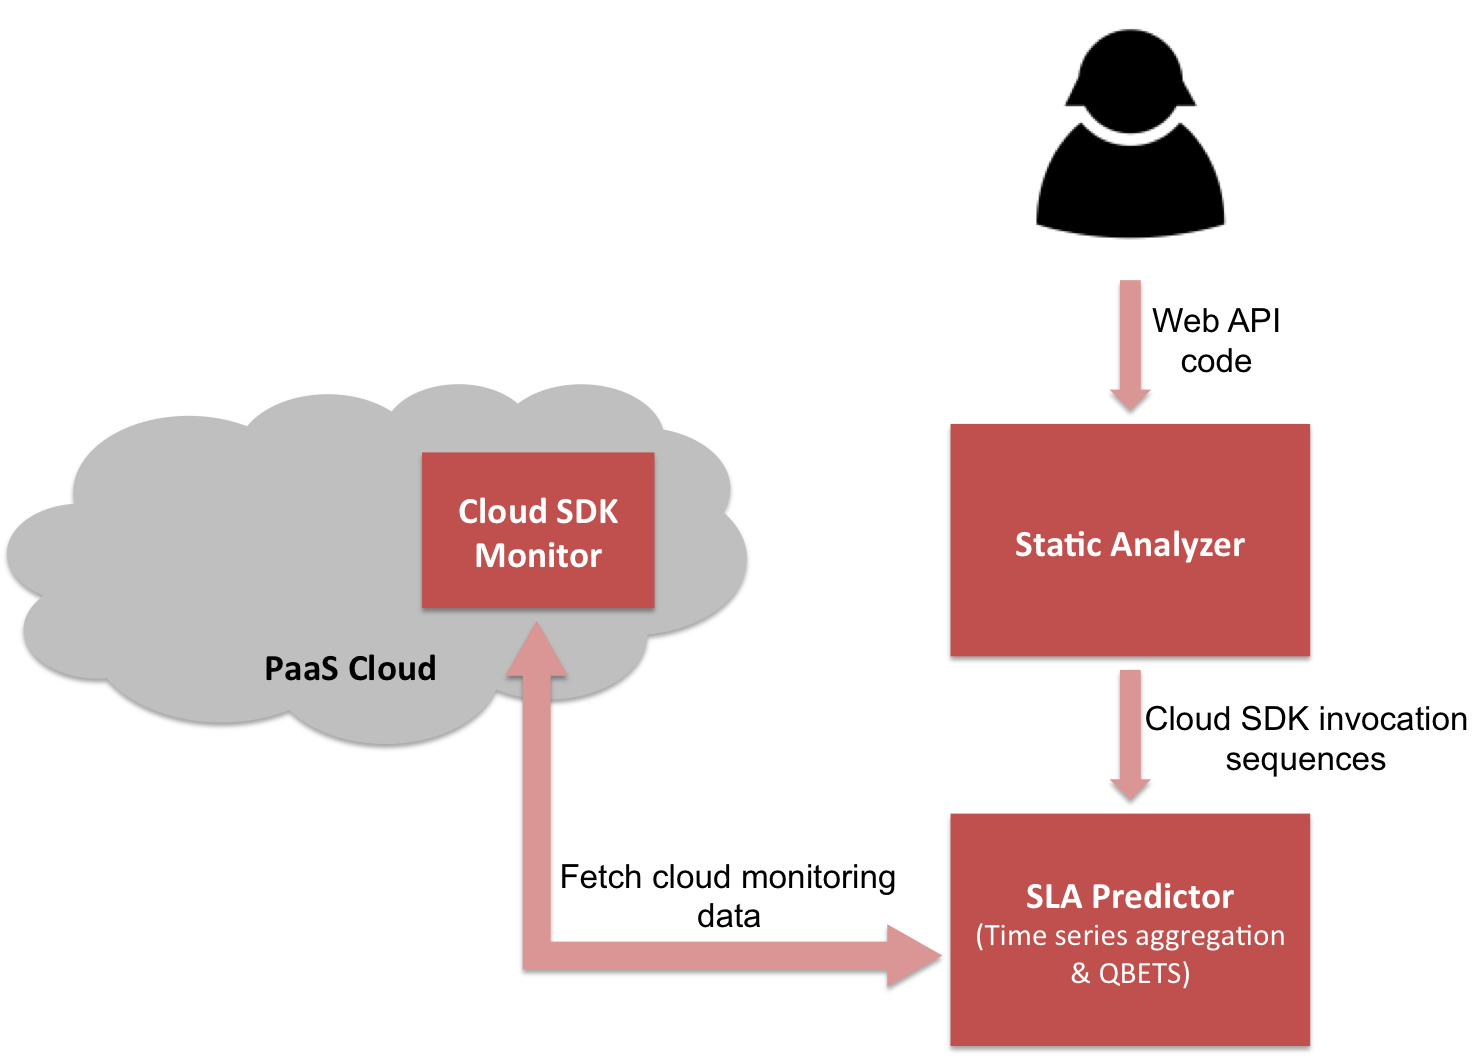
\includegraphics[scale=0.35]{cerebro_arch}
\caption{Cerebro architecture and component interactions.}
\label{fig:cerebro_arch}
\end{figure}

Figure~\ref{fig:cerebro_arch} illustrates all the components of Cerebro and how they interact with each other. 
Cerebro can be called into action by the web API developers, either at the development time or when the
API is ready to be deployed in the cloud. Developer submits the web API source code (or some intermediate
representation of it) to Cerebro, which is then processed by the static analyzer component. The static
analyzer extracts the sequences of cloud SDK invocations from the web API code, and hands them over
to the SLA predictor. SLA predictor then contacts Watchtower to retrieve the relevant cloud SDK operation
benchmark data (time series). Afterwards it aggregates the received time series data, and processes
the resulting time series using QBETS. The percentile ($p$) and the upper confidence ($c$) values needed
for the analysis can be configured into the SLA predictor permanently, or they can be passed in by the API
developer when she invokes Cerebro. 

The resulting Cerebro predictions can be used in many ways. In the simplest case they can be
used to clearly document the API SLAs, so that API consumers can stay informed about what 
type of performance to expect from the APIs they use. In a somewhat advanced context, Cerebro
predictions can guide the API developers on how to program web APIs to support highly competitive
SLAs. On the same note, the Cerebro predictions can provide cloud administrators with
useful insights regarding potential issues and performance bottlenecks in the cloud platform. In an
even more sophisticated environment, the Cerebro predictions can be used to enforce SLA-related
policies on web APIs deployed in the cloud. For example, one may implement a policy engine which ensures
that all APIs deployed in the cloud have execution times under some preferred limit. Such an implementation
can run Cerebro on web APIs as they are submitted for deployment, and reject any APIs that do not
support the required performance level.